\chapter{Research Opportunities And Challenges}

\nomenclature{}{}

\section{Introduction}

The sources primarily focus on Kolmogorov-Arnold Networks (KANs), a specific
type of neural network architecture, and their potential for scientific
discovery. They do not explicitly discuss the broader concept of AI generations
or their evolution. However, the sources offer insights into the ongoing shift
in AI research, highlighting the increasing emphasis on interpretability and
the desire to move beyond black-box models.

\section{Case Study}

\subsection{Problems Statement}

Traditional deep learning models, primarily based on Multi-Layer Perceptrons
(MLPs), have proven highly effective in various applications, yet they fall
short in addressing the needs of scientific discovery.

\begin{itemize}
    \item Lack of Interpretability: MLPs, often characterized as "black boxes," obscure
          the reasoning behind their predictions. This opacity hinders scientists from
          extracting meaningful insights about the underlying phenomena they study. While
          an MLP might accurately predict a physical quantity, it provides little
          understanding of the governing laws or the relationships between variables.
    \item Limited Incorporation of Scientific Knowledge: MLPs offer limited avenues for
          integrating prior scientific knowledge into their structure or training
          process. This disconnect prevents scientists from leveraging their domain
          expertise to guide model learning and ensure that the learned representations
          align with established scientific principles.
    \item Inefficiency in Symbolic Representation: While MLPs are universal function
          approximators, they are not designed to efficiently represent symbolic
          formulas, which are fundamental to scientific communication and understanding.
          Their distributed, weight-based representation makes it difficult to extract
          concise mathematical relationships from trained models.
\end{itemize}

This gap between the capabilities of traditional neural networks and the
requirements of scientific discovery motivates the exploration of alternative
architectures like Kolmogorov-Arnold Networks (KANs).

\clearpage

\subsection{Proposed Methodology}

The sources propose a methodology for synergizing KANs with scientific
knowledge, aiming to bridge the gap between connectionist AI and symbolic
science. The methodology involves a two-way exchange:

1. Science to KANs: Incorporating scientific inductive biases into KANs to enhance their effectiveness in scientific discovery.
2. KANs to Science: Extracting scientific insights from trained KANs to uncover hidden patterns and relationships within data.

Let's examine the key elements of this methodology:

Science to KANs: Building in Scientific Knowledge The sources present several
techniques for embedding scientific knowledge into KANs, focusing on three
levels of scientific understanding:
\begin{itemize}
    \item Important Features: Identifying the variables that significantly influence a
          phenomenon.
          \begin{itemize}
              \item Attribution Score: This metric quantifies the relative importance of input
                    variables by considering their contribution to the final output. It allows
                    scientists to pinpoint key features and potentially prune irrelevant ones,
                    leading to more compact and interpretable models.
              \item Pruning Inputs: Based on attribution scores, irrelevant input features can be
                    pruned away to simplify the model and focus on the most relevant variables.
          \end{itemize}

    \item Modular Structures: Understanding how different components of a system interact
          and contribute to the overall behavior.
          \begin{itemize}
              \item Anatomical Modularity: The physical grouping of nodes and edges in the KAN,
                    visually revealing distinct modules.
              \item Functional Modularity: Analysis of activation patterns and dependencies between
                    nodes to uncover functional relationships between variables. The sources define
                    three types of functional modularity. Separability: A function is separable if
                    it can be decomposed into independent sub-functions of input variables.
                    Generalized Separability: Relaxing separability to allow for interactions
                    between variables within sub-functions. Generalized Symmetry: Identifying
                    invariance of the function's output under transformations of input variables,
                    revealing symmetries within the system.
              \item Modularity Enforcement: Techniques for imposing specific modular structures
                    onto KANs, guided by prior scientific knowledge or hypotheses. This can involve
                    grouping variables, connecting nodes in specific ways, or constraining
                    activation function learning.
              \item Tree Converter: This tool converts trained KANs (or any neural networks) into
                    tree graphs, visualizing the hierarchical modular structure of the learned
                    function.
          \end{itemize}
    \item Symbolic Formulas: Extracting concise mathematical relationships from data.
          \begin{itemize}
              \item KAN Compiler (kanpiler): A tool that converts symbolic formulas into
                    corresponding KAN architectures. This allows scientists to embed known
                    scientific equations directly into KANs, providing a starting point for further
                    learning.
              \item Width/Depth Expansion: Techniques for expanding the width and depth of KANs
                    compiled from symbolic formulas to enhance their expressive power and allow for
                    further fine-tuning with data.
          \end{itemize}
\end{itemize}

KANs to Science: Extracting Out Scientific Knowledge The sources emphasize
three main aspects of scientific knowledge extraction from trained KANs:
\begin{itemize}
    \item Identifying Important Features: Using the attribution score, discussed earlier,
          to rank the relevance of input features and potentially guide feature selection
          or experimentation.
    \item Identifying Modular Structures: Employing the tree converter tool, along with
          techniques for detecting and analyzing different types of functional
          modularity, to reveal the hierarchical structure of the learned function and
          uncover potential sub-systems or independent mechanisms within the phenomenon
          being studied.
    \item Identifying Symbolic Formulas: Extracting symbolic formulas from trained KANs
          through a combination of techniques:
          \begin{itemize}
              \item Leveraging Modular Structures: Using the discovered modular structure to guide
                    symbolic regression by decomposing the problem into smaller, more manageable
                    sub-problems.
              \item Sparse Connection Initialization: Initializing KANs with sparse connections to
                    encourage the emergence of simpler, more interpretable representations,
                    facilitating symbolic regression.
              \item Hypothesis Testing: Training multiple KANs under different hypotheses about the
                    symbolic form of the relationship and comparing their performance to select the
                    most plausible formula.
              \item Symbolic Snapping: Converting the learned activation functions into
                    corresponding mathematical expressions using symbolic regression tools,
                    potentially with human guidance to ensure meaningfulness and interpretability.
          \end{itemize}
\end{itemize}

Applying the Methodology: Case Studies in Scientific Discovery The sources
illustrate the application of this methodology through several case studies,
demonstrating how KANs can be used to:
\begin{itemize}
    \item Discover conserved quantities in dynamical systems.
    \item Uncover hidden symmetries, such as the temporal symmetry in the Schwarzschild
          black hole metric.
    \item Learn constitutive laws in materials science, using the example of Neo-Hookean
          materials.
\end{itemize}

\clearpage

\section{Results And Discussion}

These case studies highlight the potential of KANs as a tool for scientific
discovery, showcasing their ability to uncover hidden patterns, extract
symbolic formulas, and provide insights that complement traditional scientific
methods. Conclusion: Towards Machine Learning 2.0? The sources, while
optimistic about the potential of KANs, acknowledge that they are still in
their early stages of development. They compare KANs to "software 1.0,"
emphasizing their interactivity, versatility, and focus on interpretability, in
contrast to the black-box nature of traditional deep learning, which they liken
to "software 2.0." 

Further research is needed to address challenges related to
computational efficiency, scalability, overfitting, and fairness. Nonetheless,
the proposed methodology for integrating KANs with scientific knowledge offers
a promising direction towards a more collaborative future between AI and
science, where AI systems not only predict but also explain, empowering
scientists to make fundamental discoveries.

\begin{figure}[t]
    \centering
    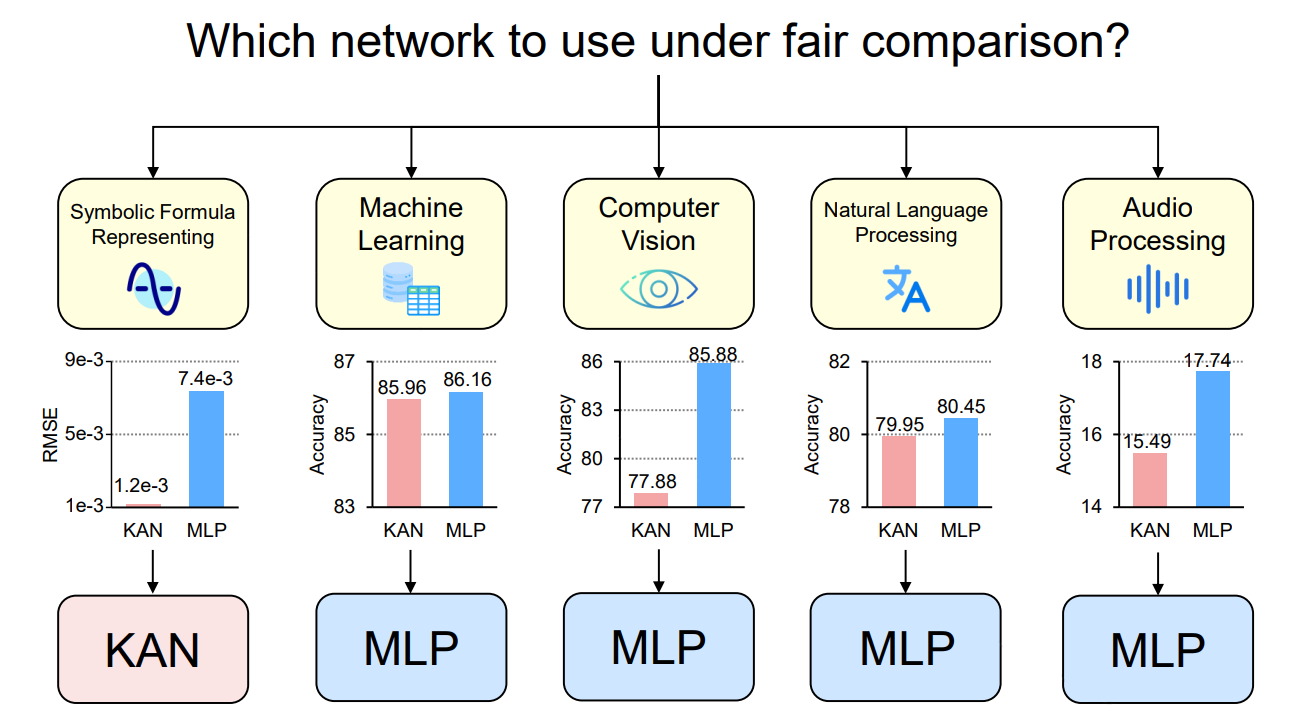
\includegraphics[width=0.9\linewidth]{Images/kan_vs_mlp.png}
    \caption{Performance comparison between KAN and MLP under fair setup. MLP yields higher
    average accuracy in machine learning, computer vision, natural language processing, and audio
    processing, while KAN leads to lower average root mean square error. For the Symbolic Formula
    Representation task, a lower RMSE is better}
    % \label{fig:kan_vs_mlp}
\end{figure}

\section{Applications}

\begin{itemize}
    \item Discovering conserved quantities in dynamical systems (e.g., energy or momentum).
    \item Uncovering hidden symmetries in physical laws or systems (e.g., temporal symmetry in the Schwarzschild black hole metric).
    \item Learning constitutive laws describing material behavior (e.g., Neo-Hookean model for elastic materials).
    \item Exploring knot theory to study relationships between knot invariants.
    \item Studying Anderson localization in disordered media (e.g., electron behavior in semiconductors).
    \item Solving partial differential equations (PDEs) as an alternative to MLPs.
    \item Graph analysis for pattern discovery in networked data.
    \item Operator learning applications for functional approximation.
    \item Analyzing tabular data and time series for scientific and industrial insights.
    \item Human activity recognition for behavioral studies.
    \item Neuroscience applications, such as modeling neural interactions.
    \item Quantum science for exploring subatomic particle behavior.
    \item Computer vision for pattern recognition and symbolic extraction.
    \item Kernel learning to enhance model generalization on complex data.
    \item Nuclear physics for understanding atomic interactions.
    \item Electrical engineering applications, like signal processing.
    \item Biology, especially in modeling biochemical interactions.
\end{itemize}

\begin{figure}[t]
    \centering
    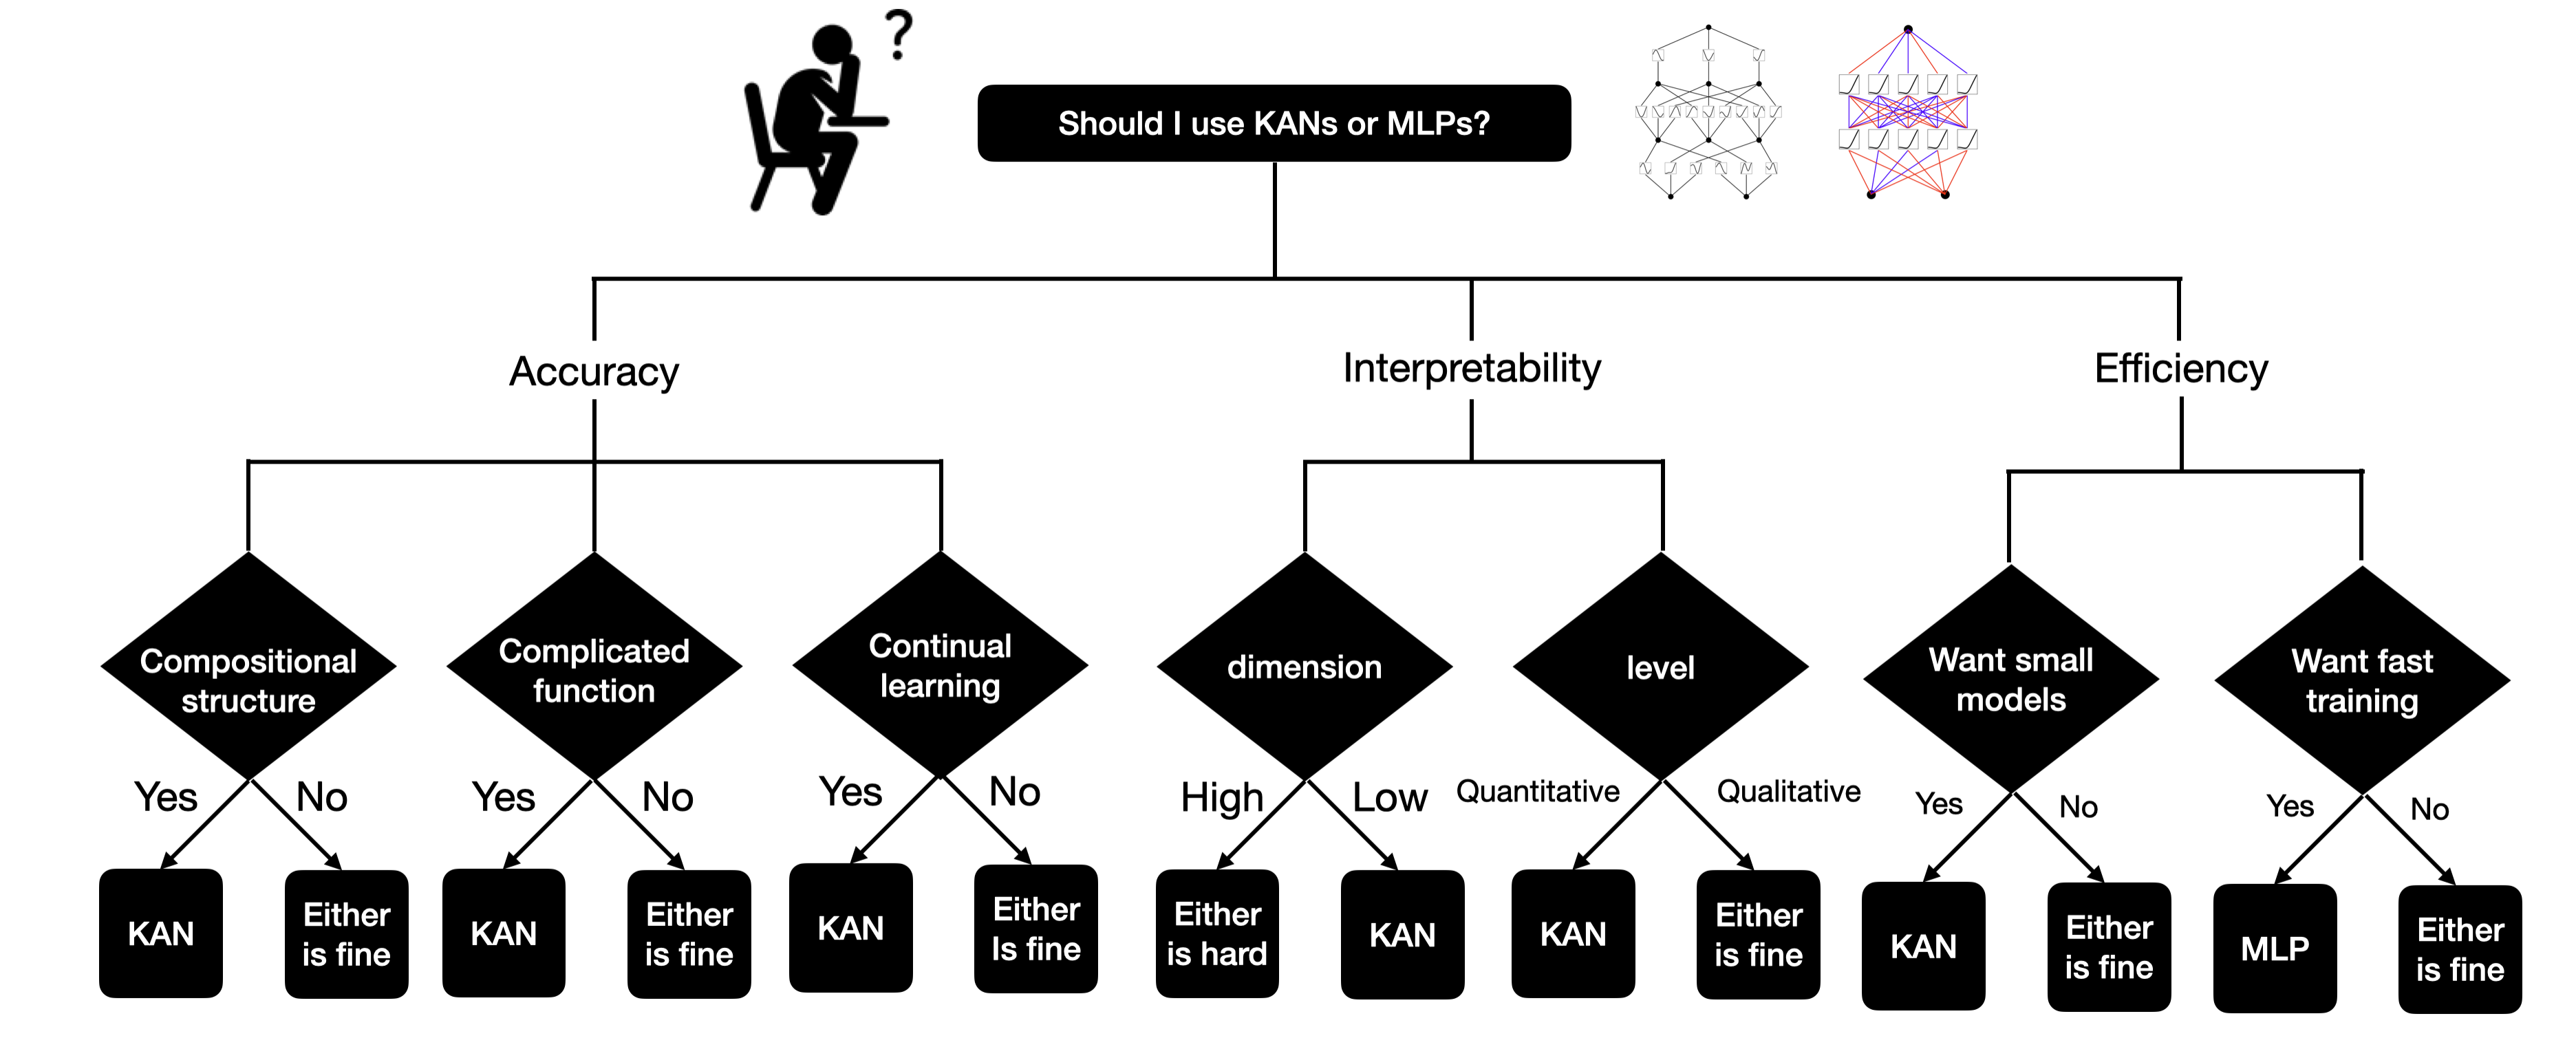
\includegraphics[width=1\linewidth]{Images/decision_tree.png}
    \caption{Should I use KANs or MLPs?}
    \label{fig:decision-tree}
\end{figure}

These applications represent potential areas where KAN models could provide novel insights or improve efficiency and accuracy in scientific and engineering fields.

\section{Challenges}

These challenges highlight the areas where further research, technical advancements, and practical guidelines are needed to refine KAN models and expand their applications.

\begin{itemize}
    \item Slow training speed compared to MLPs due to complexity in learning numerous 1D spline functions.
    \item Limited batch computation, hindering efficient parallelization and slowing training.
    \item Engineering challenges related to optimizing implementation and exploring alternative training algorithms.
    \item Decreasing interpretability as model size and complexity increase.
    \item Limitations of current interpretability methods for handling large-scale KANs.
    \item Difficulty in maintaining interpretability for large-scale models without advanced techniques.
    \item Susceptibility to overfitting, especially with noisy real-world data.
    \item Need for regularization techniques, such as sparsity-inducing penalties, to control overfitting.
    \item Ongoing debates about the fairness of comparisons with MLPs, requiring controlled experimental conditions.
    \item Mixed empirical evidence, with some studies showing that optimized MLPs can match or surpass KANs.
    \item Lack of established best practices for architecture design, activation function selection, and training.
    \item Limited exploration of KANs’ performance on sequential data, such as time series and natural language.
    \item Potential issues with local minima due to the use of spline functions, which may require sophisticated optimization.
    \item Challenges in balancing computational efficiency, scalability, and interpretability to fully realize KANs’ potential in scientific discovery. 
\end{itemize}